\documentclass[10pt]{beamer}
\usetheme[progressbar=frametitle]{metropolis}
\usepackage{booktabs}
\usepackage[scale=2]{ccicons}

\usepackage{pgfplots}
\usepgfplotslibrary{dateplot}

\usepackage{xspace}
\title{Elastic Search}
\subtitle{Seminar Presentation}
\date{\today}
\author{Mohammed Nisham}
\institute{College of Engineering, Trivandrum}
% \titlegraphic{\hfill
\includegraphics[height=1.5cm]{cet_emblem}}

\begin{document}
\nocite{*}
\maketitle

\begin{frame}{Table of Contents}
  \setbeamertemplate{section in toc}[sections numbered]
  \tableofcontents[hideallsubsections]
\end{frame}

\section{Introduction}
\begin{frame}{What is elastic search}
	\begin{itemize}
		\item Built on top of Apache Lucene
		\item Built in java, Uses RESTful APIs
		\item Users - Facebook, Github, Wikipedia
		\item Ranked first in Search engine Databases
		\item Full text search
	\end{itemize}
\end{frame}

\begin{frame}{History}
	\begin{itemize}
		\item Shay Banon created Compass library in Java
		\item Not Scalable
		\item Rebuilt in distributed approach using RESTful API
	\end{itemize}
\end{frame}

\section{Features}

\begin{frame}{Document Oriented}
	\begin{itemize}
		\item Documents as JSON object
		\item Index
		\item Type - mapping
		\item Id
		\item Dynamic mapping
	\end{itemize}
\end{frame}

\begin{frame}{Sharding}
	\begin{itemize}
		\item Distributed document store
		\item Complete Lucene search engine
		\item Primary and Replica shards
		\item Hash functions for shard routing
		\item Immutability by segments
		\item Near real timing by In-memory Buffer
		\item Crash recovery with Translog
	\end{itemize}
\end{frame}

\begin{frame}{Sharding}
	\begin{figure}
		\centering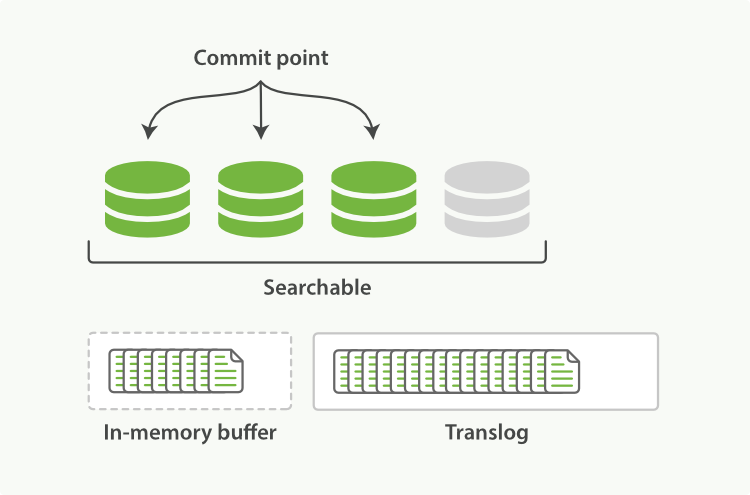
\includegraphics[width=10cm]{inside_shard}
		\caption{Inside a shard}
	\end{figure}
\end{frame}

\begin{frame}{Clustering}
	\begin{itemize}
		\item Node - instance of ES server
		\item Cluster Health
		\item Failure recovery
		\item Horizontal scaling
		\item Cluster master
		\item Completely autonomous
	\end{itemize}
\end{frame}

\begin{frame}{Clustering}
	\begin{figure}
		\centering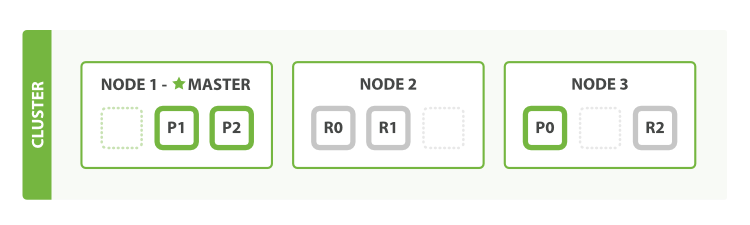
\includegraphics[width=10cm]{cluster}
		\caption{A sample cluster}
	\end{figure}
\end{frame}

\begin{frame}{Clustering}
	\begin{figure}
		\centering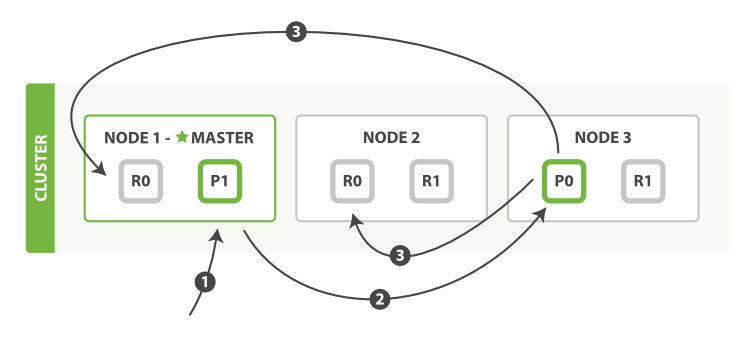
\includegraphics[width=10cm]{cluster_data}
		\caption{Request routing in a cluster}
	\end{figure}
\end{frame}

\begin{frame}{Mapping and analysis}
	\begin{itemize}
		\item Inverted index
		\item Dynamic mapping
		\item Analyzers
		\item Character filter, tokenizer and token filter
	\end{itemize}
\end{frame}

\begin{frame}{Aggregations}
	\begin{itemize}
		\item Buckets
		\item Metrics
		\item Usable with filters and queries
	\end{itemize}
\end{frame}

\begin{frame}{Concurrency}
	\begin{itemize}
		\item Optimistic concurrency control
		\item Operations are asynchronous and concurrent
		\item Metafield version
	\end{itemize}
\end{frame}


\section{Search}

\begin{frame}{Distributed search}
	\begin{itemize}
		\item Query phase
		\item Fetch phase
	\end{itemize}
\end{frame}

\begin{frame}{Distributed search}
	\begin{figure}
		\centering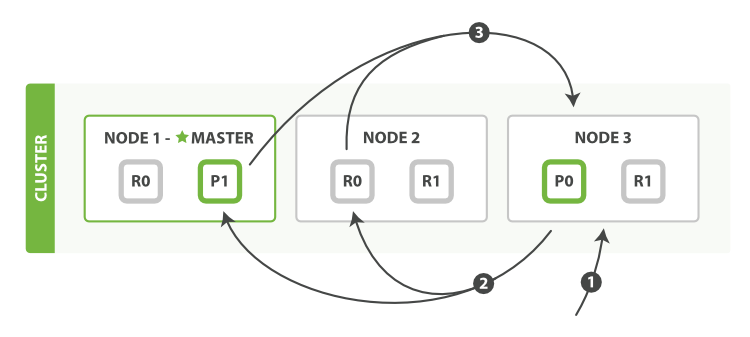
\includegraphics[width=10cm]{query_phase}
		\caption{Query phase in distributed search}
	\end{figure}
\end{frame}

\begin{frame}{Distributed search}
	\begin{figure}
		\centering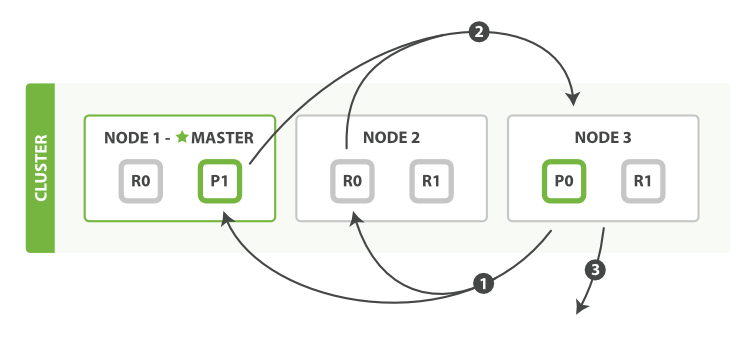
\includegraphics[width=10cm]{fetch_phase}
		\caption{Fetch phase in distributed search}
	\end{figure}
\end{frame}



\begin{frame}{Relevance}
	\begin{itemize}
		\item Score Calculation
		\item Term Frequency
		\item Inverted Document frequency
		\item Field length norm
		\item Boost
	\end{itemize}
\end{frame}

\begin{frame}{Structured search}
	\begin{itemize}
		\item Search Lite
		\item Query DSL
		\item Query and Filter
		\item Combinations
	\end{itemize}
\end{frame}

\begin{frame}{Full text search}
	\begin{itemize}
		\item Difficulties with normal DB model
		\item Multi word search
		\item Multi field search
		\item Metafield all
		\item Phrase search
		\item Search as you type, Edge n-grams
		\item Fuzzy search
	\end{itemize}
\end{frame}


\section{Conclusion}
\begin{frame}{Use}
	\begin{itemize}
		\item Real time and full text search
		\item Logging massive data - The Guardian
		\item Geolocation with full text - Stack overflow
		\item Sheer scale - Github
	\end{itemize}
\end{frame}

\begin{frame}{Performance Analysis}
	\begin{figure}
		\centering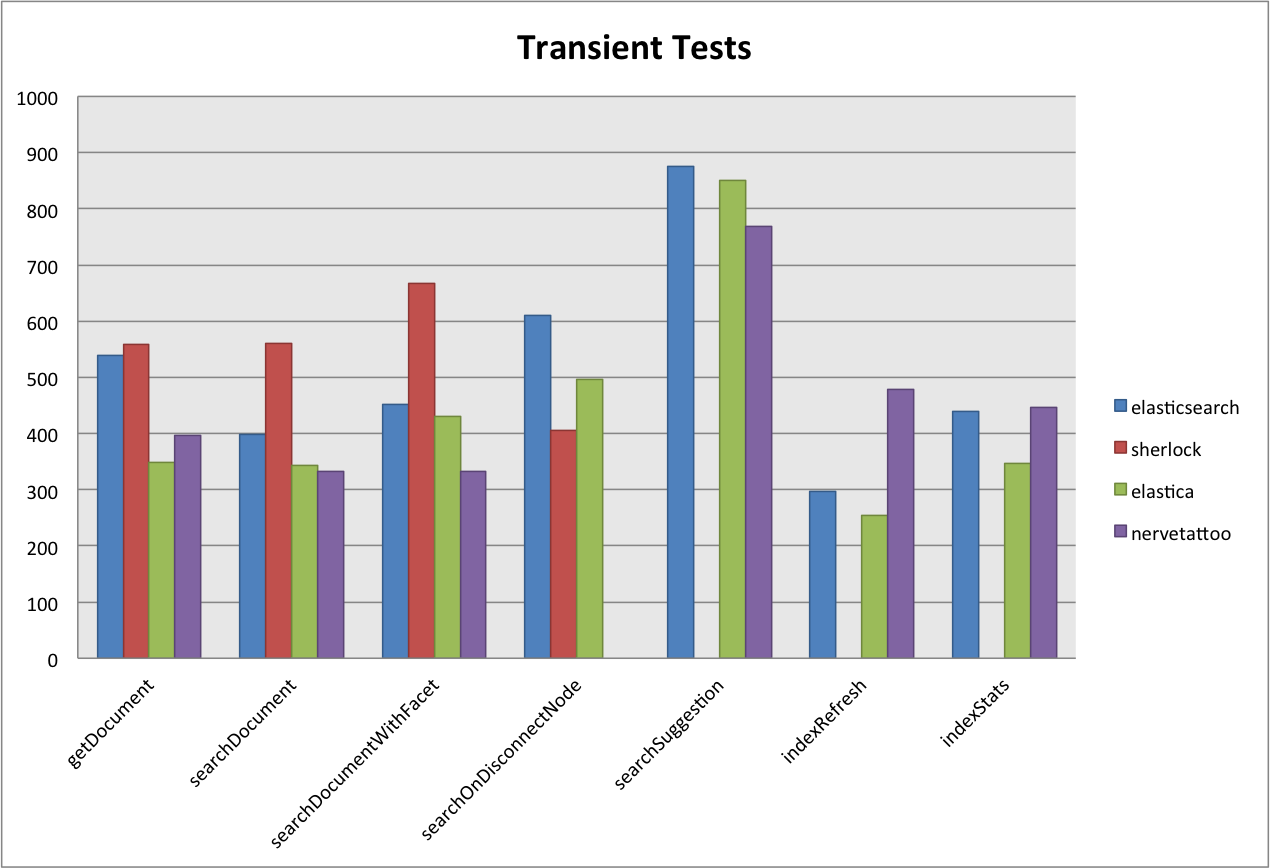
\includegraphics[width=8cm]{clients}
		\caption{Performance analysis of different PHP Clients of ES}
	\end{figure}
\end{frame}

\begin{frame}{Memory and Time Requirements}
	\begin{figure}
		\centering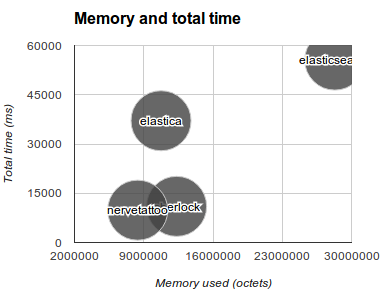
\includegraphics[width=8cm]{clients_memory}
		\caption{Memory and Time requirement of different PHP Clients of ES}
	\end{figure}
\end{frame}

\begin{frame}[standout]
  Questions?
\end{frame}

\begin{frame}[allowframebreaks]{References}

  \bibliography{../common/seminar}
  \bibliographystyle{abbrv}

\end{frame}

\end{document}